\section{Library}


\subsection{Architecture Overview}

\begin{frame}\frametitle{Architecture Overview}

%!TEX root = ../../main.tex

\begin{figure}
\caption{
    Dependency Graph of the Morpheus GraphQL Packages
    \label{fig:dependency-graph}
    }
\begin{center}
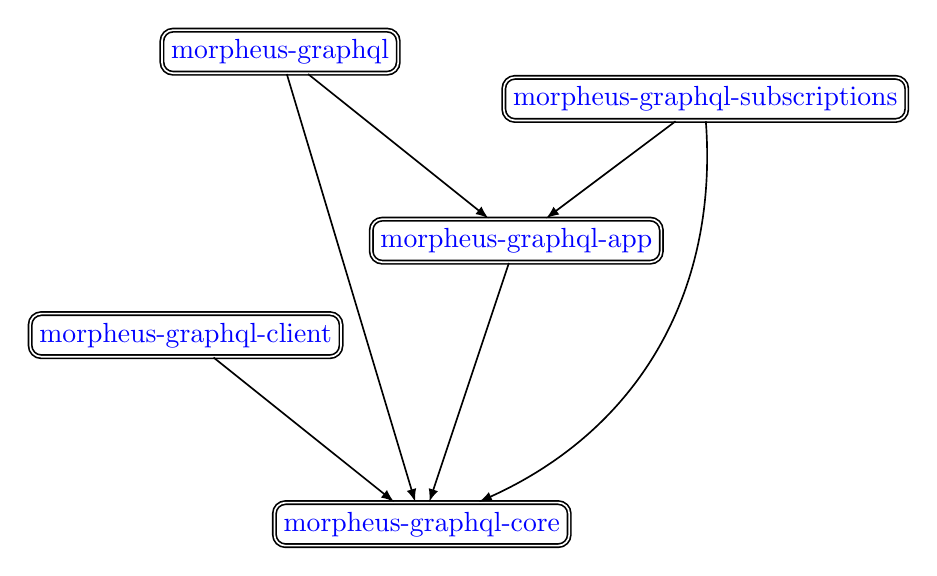
\begin{tikzpicture}[
        scale=.6,
        auto=left,
        -latex ,
        auto ,
        node distance =2 cm and 2cm ,
        % on grid ,
        semithick ,
        package/.style ={ fill=red!20,draw,double,rounded corners ,top color =white ,draw , text=blue , minimum width =1 cm},
    ] 
    \node[package] (core) at (10,0) {morpheus-graphql-core};
    \node[package] (client) at (5,4)  {morpheus-graphql-client};
    \node[package] (app) at (12,6)  {morpheus-graphql-app};
    \node[package] (server) at (7,10)  {morpheus-graphql};
    \node[package] (subs) at (16,9) {morpheus-graphql-subscriptions};
  
    \path (client) edge (core);
    \path (app)  edge (core);
    \path (server)  edge  (core);
    \path (server)  edge  (app);
    \path (subs)  edge  (app);
    \path 
        (subs) 
            edge [bend left =35] 
        (core);  

\end{tikzpicture}
\end{center}
\end{figure}

\end{frame}

\subsection{Design Decisions} 
\begin{frame}\frametitle{Design Decisions}

\begin{itemize}
    \li{Code-First Approach} A single type change automatically updates the resolver types and GraphQL schema. 
    \li{Embeded Domain Specific Language} By using the familiar syntax of the native language, users can focus on domain-specific problems~\cite{edsl-modeling}.
    \li{Datatype-Generic Programming} eliminates boilerplate code~\cite{scrap-your-boilerplate}.
    \li{Monadic Resolvers} all side effects in Haskell are performed with monads. 
    \li{Parameterized Resolver Types} Parametric polymorphism allows the modular definition of resolver types, where the type parameter determines the allowed operations.
\end{itemize}
\end{frame}

\subsection{Schema Derivation} 
\begin{frame}\frametitle{Schema Derivation}

GraphQL models the schema as a graph, where nodes are types and fields are edges~\cite{migrating-to-gql}. We use deep-first search and derive all schema types from the root node while using cycle checking to avoid loop cycles.

\end{frame}

\subsection{Mapping Rules}

\begin{frame}\frametitle{Mapping Built-in Types}
\begin{itemize}
  \li{Wrapping Types}
  \begin{itemize}
    \li{Non-Null} inverse mapping with Maybe
    \li{List} List
  \end{itemize}
  \li{Scalar Types}
  \begin{itemize}
    \li{Int} Int
    \li{Float} Double
    \li{String} Text
    \li{Boolean} Bool
    \li{ID}  defined custom data type ID 
  \end{itemize}
\end{itemize}
\end{frame}

\begin{frame}\frametitle{Mapping Type Definitions}

\begin{itemize}
  \li{Enums} data types with empty alternatives.
  \li{Input object and field arguments} data types with non-empty single constructors (records). 
  \li{Objects} We represent the object types with parameterized records, where the record fields can take function types. With this technique, types can be defined independently of the resolution operations, and the concrete operations can be passed recursively from parent to child. 
  \li{Unions} data type with multiple alternatives, where at least one alternative is non-empty.
  \begin{itemize}
    \item we create a new object for each alternative.
    \item we unpack constructors, where the name is the concatenation of the type constructor name and the referencing type name. 
    \item we assign to each empty alternate unit field.
  \end{itemize}
\end{itemize}

\end{frame}

